%
%    Template for Belle journal submissions
%
%
% TeX'ing this file requires that you have AMS-LaTeX 2.0 installed
% as well as the rest of the prerequisites for REVTeX 4.0
%
% See the REVTeX 4 README file
% It also requires running BibTeX. The commands are as follows:
%
%  1)  latex apssamp.tex
%  2)  bibtex apssamp
%  3)  latex apssamp.tex
%  4)  latex apssamp.tex
%
%%% Use this for e-print submission 
%%% You also need to do the following:
%%%   * Comment out widetext, use eqnarray and \nonumber 
%%%     (for the first line) for eq:likelihood
%%%   * Change the figure size to 0.6
%%%   * Put preprint numbers and the Belle logo
%\documentclass[aps,prl,preprint,tightenlines,superscriptaddress,showpacs,byrevtex]{revtex4}
%
%%% Use this for PRL submission 
%%% You also need to do the following:
%%%   * Comment out widetext, use eqnarray and \nonumber 
%%%     (for the first line) for eq:likelihood
%%%   * Change the figure size to 0.6
%%%   * Comment out preprint numbers and the Belle logo
%\documentclass[aps,prl,preprint,superscriptaddress,showpacs,byrevtex]{revtex4}
%
%%% Double-column style
%%% You also need to do the following:
%%%   * Use widetext for eq:likelihood, comment out \nonumber
%%%   * Change the figure size appropriately (should be less than 0.5)
%%%   * Comment out preprint numbers and the Belle logo
\documentclass[aps,prl,twocolumn,superscriptaddress,showpacs,preprintnumbers,amsmath,amssymb]{revtex4}
%

% Some other (several out of many) possibilities
%\documentclass[preprint,aps]{revtex4}
%\documentclass[preprint,aps,draft]{revtex4}

\usepackage{graphicx} % Include figure files
\usepackage{dcolumn}  % Align table columns on decimal point
\usepackage[inline]{enumitem} %To have inline lists
\usepackage[hypertex]{hyperref} % hyperlinks for references.

\graphicspath{{./Figures_and_Plots/}}

\renewcommand{\arraystretch}{1.1}

% Belle authors Checklist:
% 1) Title; use \\ to break title over several lines.
% 2) Author list
% 3) Abstract
% 4) pacs numbers, for PRL, PRD
% 5) Body

\begin{document}

%\vspace*{-3\baselineskip}
%\resizebox{!}{3cm}{\includegraphics{belle.eps}}


\preprint{\vbox{ \hbox{   }
						\hbox{Belle DRAFT {\it YY-NN}}
                        \hbox{Intended for {\it Journal name}}
                        \hbox{Author: M. Yamauchi}
                        \hbox{Committee: T. Maskawa(chair),}
                        \hbox{N. Cabibbo, M. Kobayashi, }
  		              % \hbox{hep-ex nnnn}
}}

\title{ \quad\\[1.0cm] Study of the $B^{\pm} \rightarrow [\pi^{+} \pi^{-} \pi^{0}]_{D} h^{\pm}$ $(h = K, \pi)$ decay mode for a measurement of $\phi_3$ using the GLW method}

%%%% >>>>> insert the authorlist here. BEFORE the abstract !!!!! <<<<<
%%%% >>>>> from the authorship confirmation web page
%%% Name the file author.tex and use \input{author} to insert into your latex file.
\author{Author}\affiliation{affiliation}
\collaboration{The Belle Collaboration}
\noaffiliation
%% end author list

\begin{abstract}
We present a study of the decay mode $B^{\pm} \rightarrow DK^{\pm} (D = D^{0} \mathrm{or} \bar{D^{0}})$, with the $D$ subsequently decaying to $\pi^{+} \pi^{-} \pi^{0}$. This decay is sensitive to the CP-violating parameter $\phi_{3}$. We measure the CP asymmetry, $A_{F_+}$, and the branching-fraction ratio, $R_{F_+}$, for this decay mode using the full Belle data sample of $772 \times 10^6 B\bar{B}$ pairs collected with the Belle detector at KEKB asymmetric $e^{+}$ $e^{-}$ collider to be:
\begin{align}
&A_{F_+} \equiv \frac{\Gamma(B^- \rightarrow D_{F_+}K^-) - \Gamma(B^+ \rightarrow D_{F_+}K^+)}{\Gamma(B^- \rightarrow D_{F_+}K^-) + \Gamma(B^+ \rightarrow D_{F_+}K^+)} \nonumber \\
&~~~~~~= 0.16 \pm 0.12 (\mathrm{stat.}) \pm 0.05 (\mathrm{syst.}) , \nonumber\\
&R_{F_+} \equiv \frac{\Gamma(B^- \rightarrow D_{F_+}K^-) + \Gamma(B^+ \rightarrow D_{F_+}K^+)}{\Gamma(B^- \rightarrow D^0K^-) + \Gamma(B^+ \rightarrow \bar{D}^0K^+)} \nonumber \\
&~~~~~~= 0.076 \pm 0.012 (\mathrm{stat.})  ^{+0.032} _{-0.027} (\mathrm{syst.}) \nonumber. 
\end{align}
\end{abstract}

\pacs{XX.YY.ZZ, AA.BB.CC}

\maketitle

%%%% >>>> keep the final version single-spaced
\tighten

{\renewcommand{\thefootnote}{\fnsymbol{footnote}}}
\setcounter{footnote}{0}

CP violation in the Standard Model of particle physics (SM) is governed by an irreducible complex phase in the $3 \times 3$ Cabibbo-Kobayashi-Maskawa (CKM) quark mixing matrix. Measurement of this parameter is central to the study of CP-violation in the Standard Model. However, present measurements of the angle $\phi_3$ are significantly less precise than those of the other two Unitary Triangle  (UT) angles, $\phi_1$ and $\phi_2$. The importance of arriving at a more precise estimate for $\phi_3$ lies in the fact that it is the only CP-violating parameter that can be measured using just tree-level decays, which are well understood within the context of the SM. Such a measurement can then serve as a benchmark in the search for new physics in loop-dominated processes. 

Each of the three angles of the UT can be measured independently, using one or more of the available decay modes \cite{HFAG}. In this paper, we focus on the $B^{\pm} \rightarrow [\pi^{+} \pi^{-} \pi^{0}]_{D} h^{\pm}$ $(h = K, \pi)$ decay mode. Equations \ref{eq:subeq1a} and \ref{eq:subeq1b} summarise the two GLW observables that are sensitive to $\phi_3$, namely the charge asymmetry $A_{F_+}$ and the branching fraction ratio $R_{F_+}$, where the subscript $F_+$ indicates that the $D^0/\bar{D}^0$ decays to a final state with CP-fraction $F_+$. $F_+$ takes on the value of $+1$ for a purely CP-even state, and $0$ for a purely CP-odd state. The amplitude ratio $r_B$ is defined as $\left|\dfrac{\mathcal{A}(B^- \rightarrow \bar{D}^0K^-)}{\mathcal{A}(B^- \rightarrow D^0K^-)}\right|$, and the strong phase difference $\delta_B = \delta(B^- \rightarrow \bar{D}^0K^-) - \delta(B^- \rightarrow D^0K^-)$.


\begin{subequations} \label{eq:1}
\begin{align}
&A_{F_+} = \frac{\Gamma(B^- \rightarrow D_{F_+}K^-) - \Gamma(B^+ \rightarrow D_{F_+}K^+)}{\Gamma(B^- \rightarrow D_{F_+}K^-) + \Gamma(B^+ \rightarrow D_{F_+}K^+)} \label{eq:subeq1a}\\
&=[(2F_+ -1)\cdot 2r_B \cdot \sin\delta_B\cdot\sin\phi_3]/R_{F_+} ,\nonumber \\
&R_{F_+} = \frac{\Gamma(B^- \rightarrow D_{F_+}K^-) + \Gamma(B^+ \rightarrow D_{F_+}K^+)}{\Gamma(B^- \rightarrow D^0K^-) + \Gamma(B^+ \rightarrow \bar{D}^0K^+)} \label{eq:subeq1b}\\
&=1 + r_B^2 +(2F_+ -1)\cdot 2r_B \cdot \cos\delta_B \cdot \cos\phi_3 . \nonumber 
\end{align}
\end{subequations}    

The CP-content of $D \rightarrow \pi^- \pi^+ \pi^0$ (here and elsewhere in this paper, $D$ denotes $D^0$ or $\bar{D}^0$) has been studied recently \cite{Fplus}. The measured value $F_+ = 0.969 \pm 0.018 \pm 0.005$ suggests that this final state is almost purely CP-even. This, coupled with the larger branching fraction ($1.47\%$) of $[\pi^+ \pi^- \pi^0]_D$ as compared to $[K^+ K^-]_D$ and $[\pi^+ \pi^- ]_D$ makes the decay $B^{\pm} \rightarrow [\pi^+ \pi^- \pi^0]_{D} K^{\pm}$ a good candidate for $\phi_3$ measurement using the GLW method proposed by Gronau, London and Wyler \cite{GLW}. A summary of the results from previous analyses of this decay mode is given in Table \ref{table:Table 1}. 

\begin{table}[htb]
\caption{Summary of results from other analyses of $B^{\pm} \rightarrow [\pi^+ \pi^- \pi^0]_{D} K^{\pm}$ \cite{HFAG}}
\centering
\resizebox{\columnwidth}{!}{
\begin{tabular}{c c c c} 
\hline\hline
Integrated Luminosity & $R_{F_+}$ & $A_{F_+}$ & Reference \\ [0.5ex]

$N(B\bar{B})$ = 324M & - & -0.02 \pm 0.16 \pm 0.03 & BaBar \cite{BaBar} \\
3fb^{-1} & 0.98 \pm 0.11 \pm 0.05 & 0.05 \pm 0.09 \pm 0.01 & LHCb \cite{LHCb} \\

\hline


\hline
\end{tabular}
}
\label{table:Table 1}
\end{table}

This analysis was done on a data sample of $772 \times 10^6 B\bar{B}$ pairs, collected with the Belle detector located at the KEKB asymmetric $e^+ e^-$ collider, operating near the $\Upsilon (4S)$ resonance. The principal sub-detectors relevant to this analysis are a silicon vertex detector (SVD), a 50-layer central drift chamber (CDC), an array of aerogel threshold Cherenkov counters (ACC), a barrel-like arrangement of time-of-flight scintillation counters (TOF), and an electromagnetic calorimeter consisting of $CsI(Tl)$ crystals located inside a superconducting solenoid coil that provides a 1.5T magnetic field. 

 The event reconstruction procedure begins with identifying well-measured $K^{\pm}$, $\pi^{\pm}$, and $\pi^0$ candidates, which are then used to reconstruct $D \rightarrow \pi^+ \pi^- \pi^0$ events. Charged track selection for the final state particles (FSPs) is done after applying impact parameter cuts $|dr| < 0.2 ~ \mathrm{cm}$ and $|dz| < 1.5 ~ \mathrm{cm}$ (where $dr$ and $dz$ are the distances of closest approach to the IP in the $x-y$ plane and along the $z-$axis respectively). Particle identification (PID) information from the TOF, ACC and CDC are used to identify charged hadrons (i.e. $K^{\pm}$ and $\pi^{\pm}$. A likelihood-ratio cut on $L(K/\pi) = L_K/(L_K + L_{\pi})$, where $L_{\pi}$ and $L_K$ are the values of the individual likelihood functions for the charged pion and kaon PID hypotheses respectively. The requirements on $L(K/\pi)$ are $L(K/\pi) \geq 0.6$ for kaons, and $L(K/\pi) \leq 0.4$ for pions. For $\pi^0$ reconstruction, we require that the energy of the photon detected in the ECL satisfy $E_{\gamma} > 100 ~ \mathrm{MeV}$ for $12.5^o \leq \theta \leq 31^o$ (front endcap), $E_{\gamma} > 50 ~ \mathrm{MeV}$ for $33^o \leq \theta \leq 128^o$ (barrel) and $E_{\gamma} > 150 ~ \mathrm{MeV}$ for $131^o \leq \theta \leq 155^o$ (rear endcap). Additionally, we require that the momentum of the $\pi^0$ candidate in the center-of-mass (CoM) frame is greater than $0.4~ \mathrm{GeV/}c$. It is also required that the invariant mass of the pair of photons used to reconstruct the $\pi^0$ candidate, $M_{\gamma \gamma}$, satisfies $0.119 ~ \mathrm{GeV/}c^2 \leq M_{\gamma \gamma} \leq 0.146 ~ \mathrm{GeV/}c^2$, which corresponds to approximately $\pm 2.5 \sigma$ in resolution about the nominal $\pi^{0}$ mass of $0.134 ~ \mathrm{GeV/}c^2$. A mass constrained fit is applied before they are used in the reconstruction of the $D$ meson.

Neutral $D$ meson candidates are reconstructed by combining a $\pi^0$ candidate with a pair of oppositely charged pion candidate tracks. Before performing a mass constrained fit so as to improve the four-momentum resolution of the daughter particles, a cut is applied on the sum of their invariant masses ($M_{\mathrm{FSP}}$) such that $1.1 ~ \mathrm{GeV/}c^2 \leq M_{\mathrm{FSP}} \leq 2.6 ~ \mathrm{GeV/}c^2$. The signal window is then defined as $1.78 ~ \mathrm{GeV/}c^2 \leq M_{\mathrm{FSP}} \leq 1.923 ~ \mathrm{GeV/}c^2$, corresponding to 3 $\sigma$ about the mean $D$-mass. 

The $D$ candidates thus reconstructed are then combined with a charged kaon or pion to obtain a $B^{\pm} \rightarrow DK^{\pm}$ or $B^{\pm} \rightarrow D\pi^{\pm}$ candidate. Signal events are identified using the energy difference, $\Delta E$ and the beam-constrained mass, $M_{bc}$, defined in the CoM frame as $\Delta E = E_B - E_{beam}$ and $M_{bc} = \sqrt{E^2_{beam}-|\vec{p}_B|^2}$. Here, $E_{beam}$ is the beam energy, while  $E_B$ and $\vec{p}_B$ are the energy and three-momentum of the $B$ meson candidate respectively. The cuts used are $5.27 ~ \mathrm{GeV/}c^{2} < M_{bc} < 5.29 ~ \mathrm{GeV/}c^2$ and $-0.1~ \mathrm{GeV} < \Delta E < 0.2 ~ \mathrm{GeV}$.

Two important sources of background for this analysis were $(i)$ events in which the neutral $D$ meson candidate actually originates from the decay $D^{*\pm} \rightarrow D\pi^{\pm}$ in $e^+ e^- \rightarrow c\bar{c}$, and $(ii)$ $B^{\pm} \rightarrow$ [K^0_S \pi^0]_D K^{\pm}$, with the $K^0_S$ then decaying as $K^0_S \rightarrow \pi^+ \pi^-$. To suppress the former, we define a variable $\Delta M$ as the mass difference between the $D^{*\pm}$ and $D^{0}$ candidates. The $D^{*\pm}$ candidate is reconstructed from the $D^0$ candidate by combining it with a $\pi^{\pm}$ candidate that is \textit{not} used in the $B^{\pm}$ candidate reconstruction. In order to reject the $c\bar{c}$ background, we require that $\Delta M > 0.15 \mathrm{Gev/c^2}$. The $K_S^0$ background is of particular importance as the final state has opposite CP relative to the signal mode. We define the invariant mass of the charged pion pair in the final state as $M_{\pi \pi}$. We reject all decays in which $|M_{\pi \pi} - M_{K_S^0}| < 0.01~ \mathrm{GeV/}c^2$, where $M_{K_S^0} = 0.497614 ~ \mathrm{GeV/}c^2$ is the nominal mass of $K_S^0$. The cutoff of $0.01 ~ \mathrm{GeV}$ was chosen as a round number corresponding to approximately $3\sigma$, where $\sigma = 0.00318 ~ \mathrm{ GeV/}c^2$ is the standard deviation of a Gaussian fit to the $M_{\pi \pi}$ distribution for truth-matched $ $B^{\pm} \rightarrow$ [K^0_S \pi^0]_D K^{\pm}$ events. It was verified that having this veto in place did not significantly affect the $F_+$ parameter for the $D \rightarrow \pi^+ \pi^- \pi^0$ final state \cite{Chris}. This verification was carried out by using the \textit{BABAR} amplitude model to estimate the value of $F_{+}$ with and without the excluded $M_{\pi \pi}$ window. There was negligible shift in the value of $F_{+}$ between these two calculations, especially in quadrature with the other uncertainties on $F_{+}$ due to statistical and systematic sources of error. The performance of the veto was satisfactory, with almost 98\% of the background events vetoed, while only 2\% of signal events were rejected.

The dominant source of background after implementing the previously defined cuts and vetoes described for this analysis is $e^+ e^- \rightarrow q\bar{q}$, where $q = u, d, s$ or $c$ (continuum events). In $e^+ e^- \rightarrow \Upsilon(4S) \rightarrow B\bar{B}$ events, the $B\bar{B}$ pairs are produced nearly at rest in the Center of Mass (CoM) frame, and hence, their decay products are expected to be uniformly distributed on a sphere. However, for continuum events, the quark pairs produced are highly boosted in the CoM frame, and hence, the hadrons produced from their fragmentation are collimated about the direction of flight, leading to jet-like events. This topological difference, along with a host of other discriminating variables, are fed into a Neural Network (NN) that discriminates between continuum events and $B\bar{B}$ events. 

We used the following eight variables as inputs to the NN to discriminate between signal and background events: 
\begin {enumerate*} [label=\itshape\arabic*\upshape)]
\item the likelihood ratio ofthe Fisher discriminant formed from 17 modified Fox-Wolfram moments \cite{Wolfram}, \item the difference between the sum of charges of particles in the hemisphere about the $D$ candidate direction, and that in the opposite hemisphere, excluding particles used in the $B$ meson reconstruction, \item the product of the charge of the $B$ candidate and the sum of the charges of all kaons associated with that event \textbf{not} used in the reconstruction of the $B$ candidate, \item the cosine of the angle between the $B$ candidate flight direction and the beam axis, \item the vertex separation between the vertex marking the origin of the $B$ decay, and the remaining tracks, \item the absolute value of the cosine of the angle in the CoM frame between the thrust axis of the $B$ decay and that of other particles in the event, \item the absolute value of the $B$ flavor tagging dilution factor \cite{Bdilution}, and \item the cosine of the angle between the daughter $\pi^+$ meson's flight direction and the opposite direction to the $B$ meson in the $D$ meson's rest frame.
\end {enumerate*}

The NeuroBayes (NB) package \cite{Feindt} was used to implement the continuum suppression NN. The network was trained using samples of truth-matched signal and continuum Monte-Carlo (MC) data, after applying all of the other selection cuts previously described. The output of the NN, $\mathcal{C}_{NB}$, takes on values between $-1$ and $1$, where a value of $1 (-1)$ indicates a signal- (continuum-) like event. In this analysis, we require that $\mathcal{C}_{NB} > 0.3$, a threshold chosen so as to maximize the statistical significance of the signal, defined as $\sqrt{2 \ln \mathcal{L}_{\mathrm{sig}} - 2 \ln \mathcal{L}_{\mathrm{0}}}$, where $\mathcal{L}_{\mathrm{sig}}$ and $\mathcal{L}_{\mathrm{0}}$ are the values of the likelihood function for optimal signal yield and zero signal yield respectively (defined in Equation \ref{eq:4}). 

The distribution of the output variable from the NN is sharply peaked towards $1$ and $-1$ for signal and continuum events respectively, making it difficult to describe these distributions using analytical probability density functions (PDFs). Since signal extraction is done by means of an extended maximum likelihood fit, it is desirable to have simple analytical PDFs, such as Gaussians and Bifurcated Gaussians, describe the output of the NN. In order to achieve this, $\mathcal{C}_{NB}$ is transformed to $\mathcal{C}_{NB}'$ according to the relation

\begin{equation}
\label{eq:2
}
\mathcal{C}_{NB}' = \log \Big{(}\frac{\mathcal{C}_{NB} - \mathcal{C}_{NB,low}}{\mathcal{C}_{NB,high} - \mathcal{C}_{NB}}\Big{)},
\end{equation}

\noindent where $\mathcal{C}_{NB,low}$ is the lower cutoff placed on the NN output as described earlier, and $\mathcal{C}_{NB,high}$ is the largest value of $NB$ for all events in the dataset.

Even after implementing all selection cuts and vetoes described thus far, it is possible that there are multiple $B$ meson candidates per event. For this analysis, we only consider a single candidate per event, and hence, for events in which multiple candidates are identified, a single candidate needs to be chosen. We adopt an approach in which the best candidate is selected on the basis of minimum $\chi^2$, as defined in Equations \ref{eq:subeq3a} and \ref{eq:subeq3b}.

\begin{subequations} \label{eq:3}
\begin{align}
&\chi^2 = \big( \frac{M_D - \mu_D}{\sigma^+_D} \big)^2 +  \big( \frac{M_{bc} - \mu_{bc}}{\sigma_{bc}} \big)^2  ~, \text{for} ~ M_D > \mu_D, \text{and} \label{eq:subeq3a}\\
&\chi^2 = \big( \frac{M_D - \mu_D}{\sigma^-_D} \big)^2 + \big( \frac{M_{bc} - \mu_{bc}}{\sigma_{bc}} \big)^2  ~, \text{for} ~ M_D < \mu_D, \label{eq:subeq3b}
\end{align}
\end{subequations}

\noindent where $\mu_D ~ (\sigma^{\pm}_D)$ is the mean (width) of the distribution of the mass of the $D$ meson candidates, and $\mu_{bc} ~ (\sigma_{bc})$ is the mean(width) of the $M_{bc}$ distribution. These parameters are determined from a dataset of truth-matched signal-like MC events passing all other selection criteria and vetoes. We adopted a counting method, with the widths being determined by requiring that 68\% of the total events lie between $\mu_D - \sigma^-_D \leq M_D \leq \mu_D + \sigma^+_D$, and similarly for $M_{bc}$. The width of $M_{bc}$ was symmetrized by taking the arithmetic mean of the left and right $\sigma$s. The final set of values used was: $\mu_{bc} = 5.27883 ~\mathrm{GeV/}c^2$, $\sigma_{bc} = 2.9297 ~\mathrm{MeV/}c^2$, $\mu_{D} = 1.86285 ~\mathrm{GeV/}c^2$, $\sigma_{D}^- = 20.9471 ~\mathrm{MeV/}c^2$, and $\sigma_{D}^+ = 15.5749 ~\mathrm{MeV/}c^2$.

A useful figure of metit to gauge the performance of BCS is the ratio of fully truth-matched events to non-truth-matched events in a given MC sample, denoted by $\mathcal{F}$. In one such MC sample,
 $\mathcal{F} = 5.746 $ before BCS, while it improves to $\mathcal{F} = 8.873$ after BCS, suggesting that the BCS routine is performing as desired. Furthermore, it was found that our BCS metric selects the correct (truth-matched) candidate $\frac{165728}{169807} = 97.6 \%$ of the time. 

Another relevant parameter of interest is the reconstruction efficiency, which is the ratio of the number of truth-matched, selected events (after applying all selection cuts, continuum suppression, and best candidate selection) to the generated number of events. For the final, optimized reconstruction routine used, the reconstruction efficiency for the decay channel $B^{\pm} \rightarrow [\pi^+ \pi^- \pi^0]_{D} K^{\pm}$ was $(11.05 \pm 0.03) \%$, while that for $B^{\pm} \rightarrow [\pi^+ \pi^- \pi^0]_{D} \pi^{\pm}$ was $(11.12 \pm 0.04) \%$, as determined from a generated sample of 1,500,000 events and 500,000 events respectively (the errors cited are the statistical error, computed as $\sqrt{\mathcal{E}(1-\mathcal{E})/N}$, $\mathcal{E} =$ reconstruction efficiency, $N =$ number of generated MC events).

In order to extract the signal yield from the dataset after all selection cuts and vetoes have been applied, an extended Maximum Likelihood (ML) fitting approach is adopted. Among the various estimation methods available, the ML approach has the advantage that under certain conditions, it can saturate the Cramer-Rao bound, which means that we cannot extract any more information from the data sample. Moreover, it is asymptotically consistent. However, it is also susceptible to yielding \textit{biased} estimates, and this limitation has to be kept in mind when analyzing the systematic errors incurred (the ML estimate is, however, an asymptotically unbiased one). 

\begin{equation}
\label{eq:4}
\mathcal{L}(x_1, \ldots, x_n;\Theta) = f(x_1, \ldots, x_n;\lambda) = \prod\limits_{i=1}^{n}f(x_i;\Theta).
\end{equation}

In the context of this analysis, the observables $x_i$ are the values of the fitted variables, $\Delta E$ and $\mathcal{C}_{NB}'$, while the parameters $\lambda$ characterize the PDFs that describe various components of the composite model, and their yields. Performing the fit in two dimensions using two weakly correlated variables, $\Delta E$ and $\mathcal{C}_{NB}'$, has the advantage that the probability of wrongly identifying a background event as signal is reduced, given that two variables have to \textit{simultaneously} peak for an event to be considered signal.

For the signal extraction performed in this analysis, all selected events were grouped into one of the following categories: 
\begin {enumerate*} [label=\itshape\arabic*\upshape)]
\item $D\pi$ signal, for which $\Delta E$ was described by two Gaussians with different means and $\mathcal{C}_{NB}'$ is described by a Bifurcated Gaussian, \item $DK$ signal, for which $\Delta E$ was described by two the same two Gaussians used for the $D\pi$ signal, with the width of the auxiliary Gaussian fixed to $0.043241 \times$ the area fraction of the two Gaussians (a value fixed from MC studies), and $\mathcal{C}_{NB}'$ is described by a Bifurcated Gaussian with same widths as for $D\pi$ signal, but with its mean floated, \item $D\pi$ identified as $DK$ and $DK$ identified as $D\pi$ crossfeed backgrounds, for which the $\Delta E$ and $\mathcal{C}_{NB}'$ shapes are identical to their signal counterparts, \item A generic $B\bar{B}$ background, with $\Delta E$ modelled by a second order Chebyshev polynomial (Exponential) for $D\pi$ ($DK$) events and $\mathcal{C}_{NB}'$ modeled by a Bifurcated Gaussian, and finally, \item A generic $q\bar{q}$ background, with $\Delta E$ modeled by a second (first) order Chebyshev polynomial for $D\pi$ ($DK$) events, and $\mathcal{C}_{NB}'$ modeled by two Gaussians with different means.
\end {enumerate*}

The suitability of each of these shapes was first validated on MC samples. Shape parameters for the crossfeed background $\Delta E$ components, the $B\bar{B}$ background $\mathcal{C}_{NB}'$ components, and the ratio of the area fraction of the two Gaussians to the width of the auxiliary Gaussian for the $D\pi$ signal $\Delta E$ component were fixed to their values from MC samples. The $q\bar{q}$ background $\mathcal{C}_{NB}$ component shape parameters were fixed from the $M_{bc}$ sidebands, $5.245 ~ \mathrm{GeV/}c^{2} < M_{bc} < 5.265 ~ \mathrm{GeV/}c^2$.

The fit is performed jointly on $D\pi$ and $DK$ events. The $B^{\pm} \rightarrow Dh^{\pm}$ ($h = K, \pi$) data sample is grouped into 4 sub-samples on the basis of the charge of the $B$ candidate $\eta = \pm 1$, and a PID variable that takes on values $p (f)$ if it passes (fails) a charged kaon identification ($KID$) test ($KID > 0.6$ is classified as $p$). These sub-samples are then fitted simultaneously. Both the pion misidentification rate $\kappa =  0.0447$ and the true kaon identification efficiency $\epsilon = 0.8541$ are fixed to the values for MC data samples as determined in \cite{BN1201}. The charge asymmetries $A^{D\pi}$, $A^{DK}$, and $A^{B\bar{B}}$ (for $DK$ from $B\bar{B}$) are floated in the final fit, while those for the $D\pi$ from $B\bar{B}$ and $q\bar{q}$ components are fixed to 0. Given that the correlation between the $\Delta E$ and $NB'$ variables is small, the joint PDF for each component is arrived at by taking the product of the PDFs for each variable, and summing up these products for the various components. 

The signal yields for the simultaneous fit can be expressed as follows (in these equations, $N_{tot}^{D\pi}$ refers to the \textit{total} number of $B^{\pm} \rightarrow D\pi^{\pm}$ events, while $R_{K/\pi}$ is the ratio of branching fraction of the $B^{\pm} \rightarrow DK^{\pm}$ decay mode to that of the $B^{\pm} \rightarrow D\pi^{\pm}$ decay modes):

\begin{subequations} \label{eq:5}
\begin{align}
&DK \text{ signal ~~:}N^{DK}_{\eta, p} = \frac{1}{2}(1-\eta A^{DK})N^{D\pi}_{tot}R_{K/\pi}\epsilon ,\\
&DK \text{ in } D\pi \text{ crossfeed :} \nonumber \\
& ~~~~ N^{DK}_{\eta, f} = \frac{1}{2}(1-\eta A^{DK})N^{D\pi}_{tot}R_{K/\pi}(1- \epsilon), \\
&D\pi \text{ in } DK \text{ crossfeed :} N^{D\pi}_{\eta, p} = \frac{1}{2}(1-\eta A^{D\pi})N^{D\pi}_{tot} \kappa,\\
&D\pi \text{ signal ~~:} N^{D\pi}_{\eta, f} = \frac{1}{2}(1-\eta A^{D\pi})N^{D\pi}_{tot}(1 - \kappa).
\end{align}
\end{subequations}

Projections of the fit on the full Belle dataset are shown in Figure \ref{fig:Figure 1}. The $\chi^2/DoF$ values are indicative of good fits, while the fitted values of the physics parameters are in excellent agreement with the expectations from the study of Generic MC data. These values are reflected in Equation \ref{eq:6}.


\begin{subequations} \label{eq:6}
\begin{align}
&A_{F_{+}} =  0.16 \pm 0.12 (\mathrm{stat.}) ,\\
&R_{F_{+}} = 0.076 \pm 0.012 (\mathrm{stat.}) .
\end{align}
\end{subequations}
  

\begin{figure}

\centering
\mbox{\subfigure[]{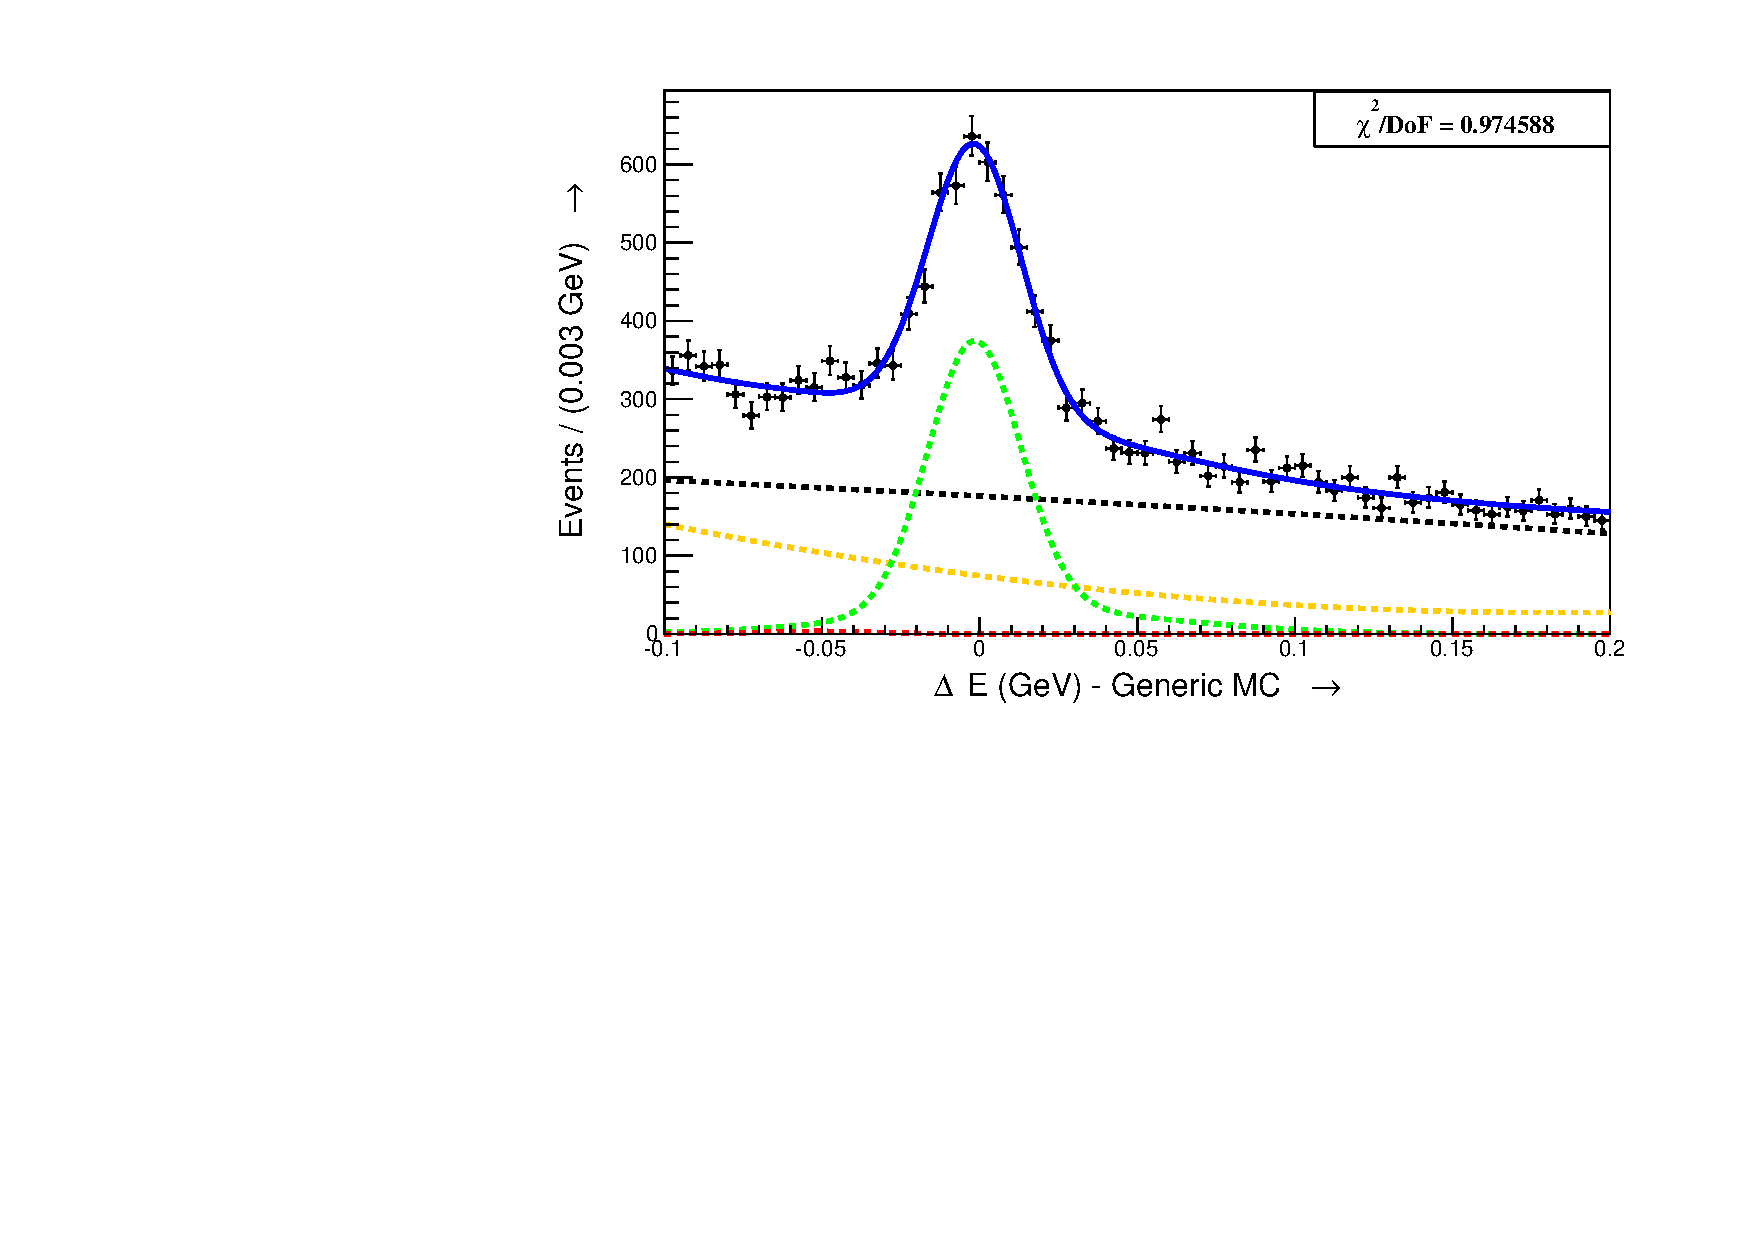
\includegraphics[width=1.5in]{data_Dpip_DE.pdf}}\quad
\subfigure[]{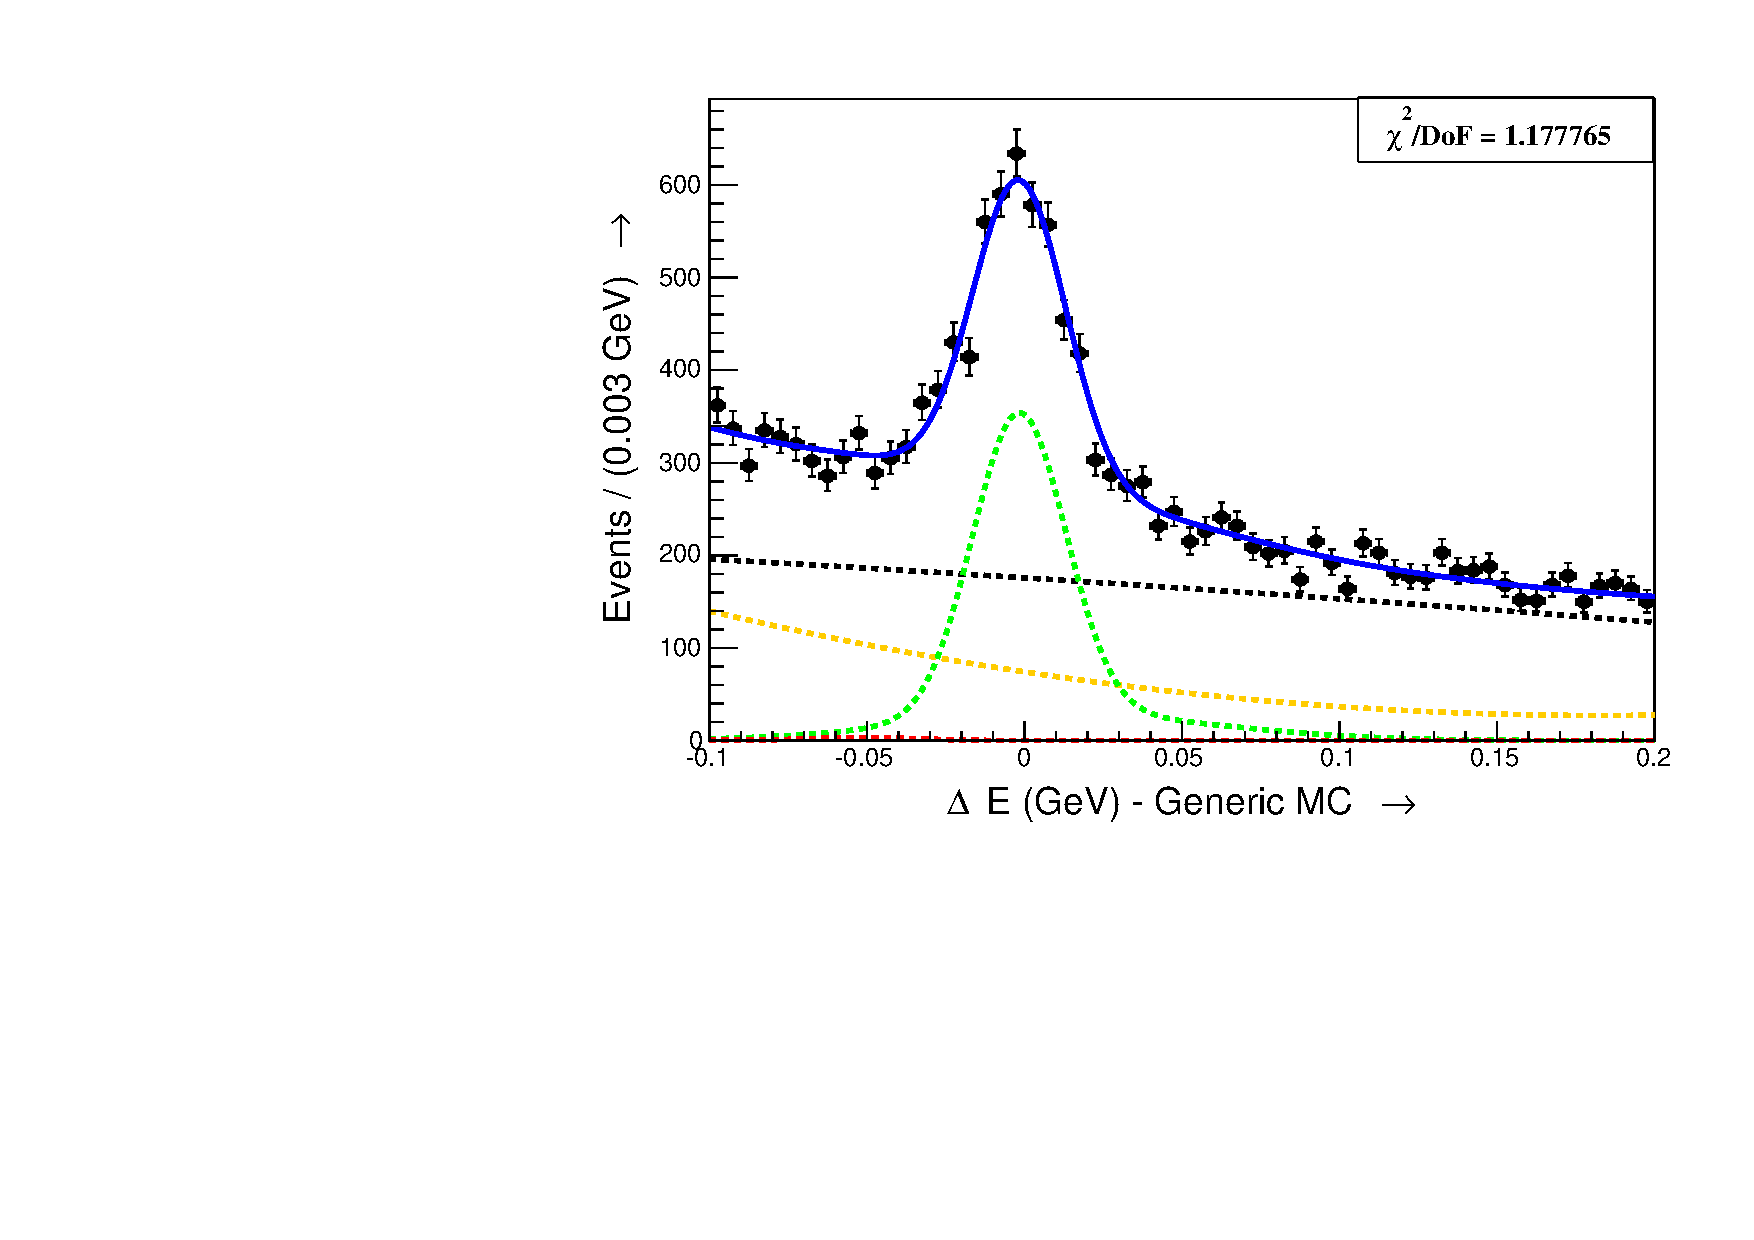
\includegraphics[width=1.5in]{data_Dpim_DE.pdf} }}

\mbox{\subfigure[]{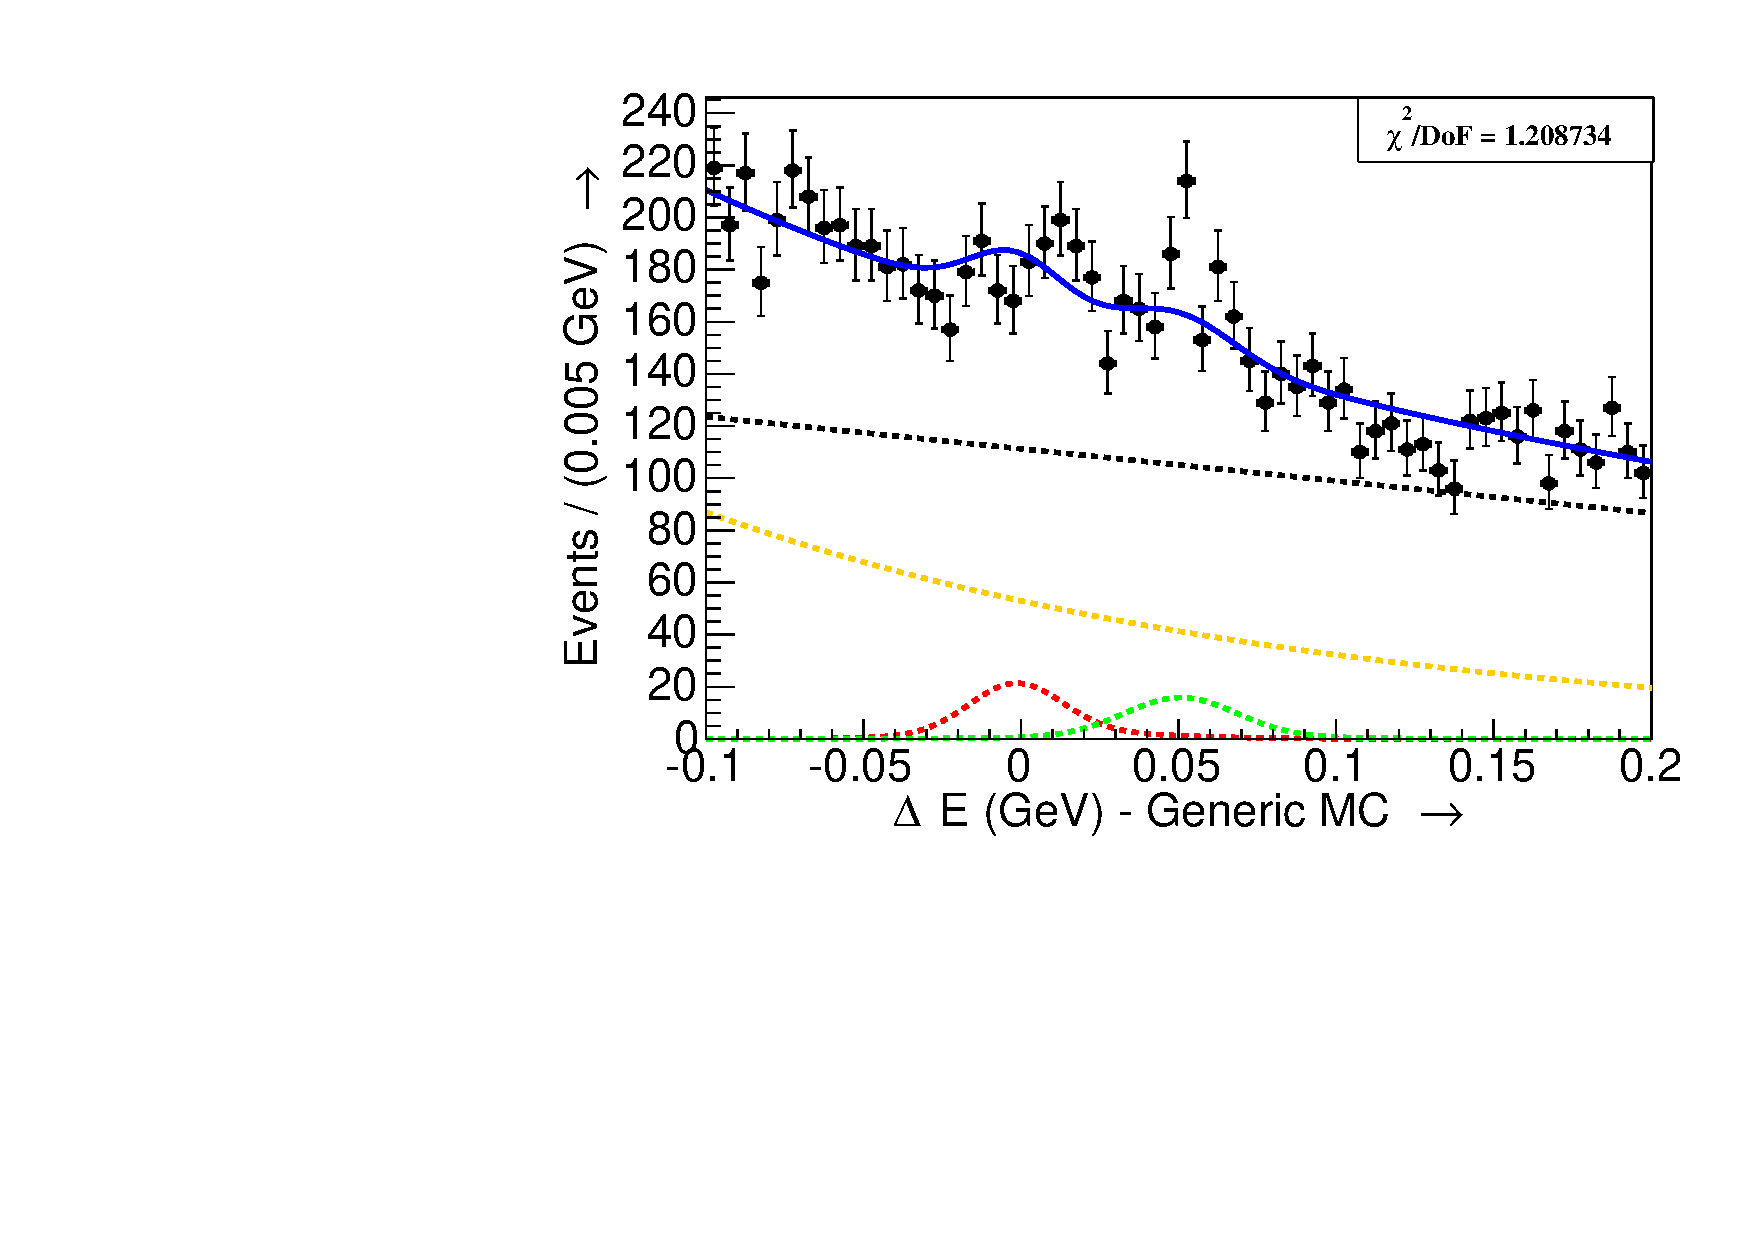
\includegraphics[width=1.5in]{data_DKp_DE.pdf}}\quad
\subfigure[]{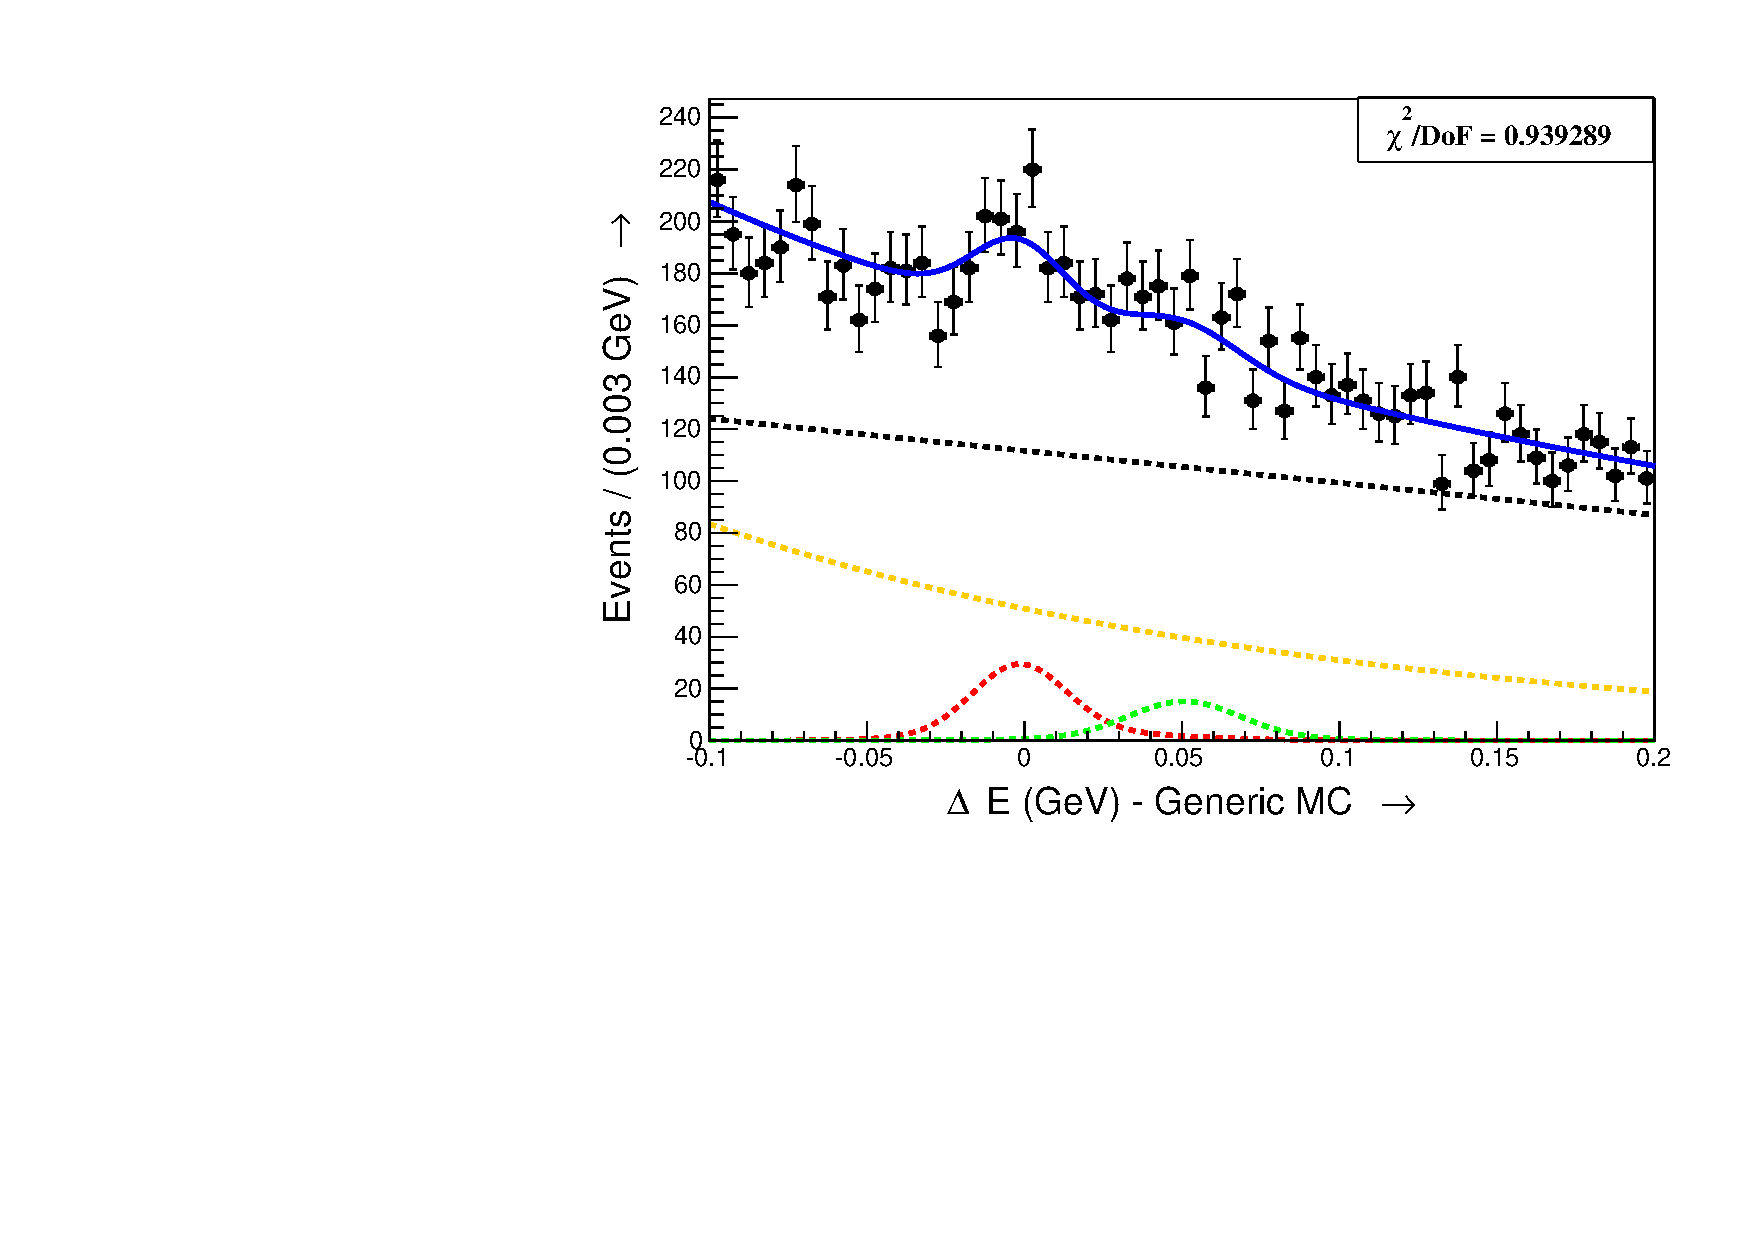
\includegraphics[width=1.5in]{data_DKm_DE.pdf} }}

\mbox{\subfigure[]{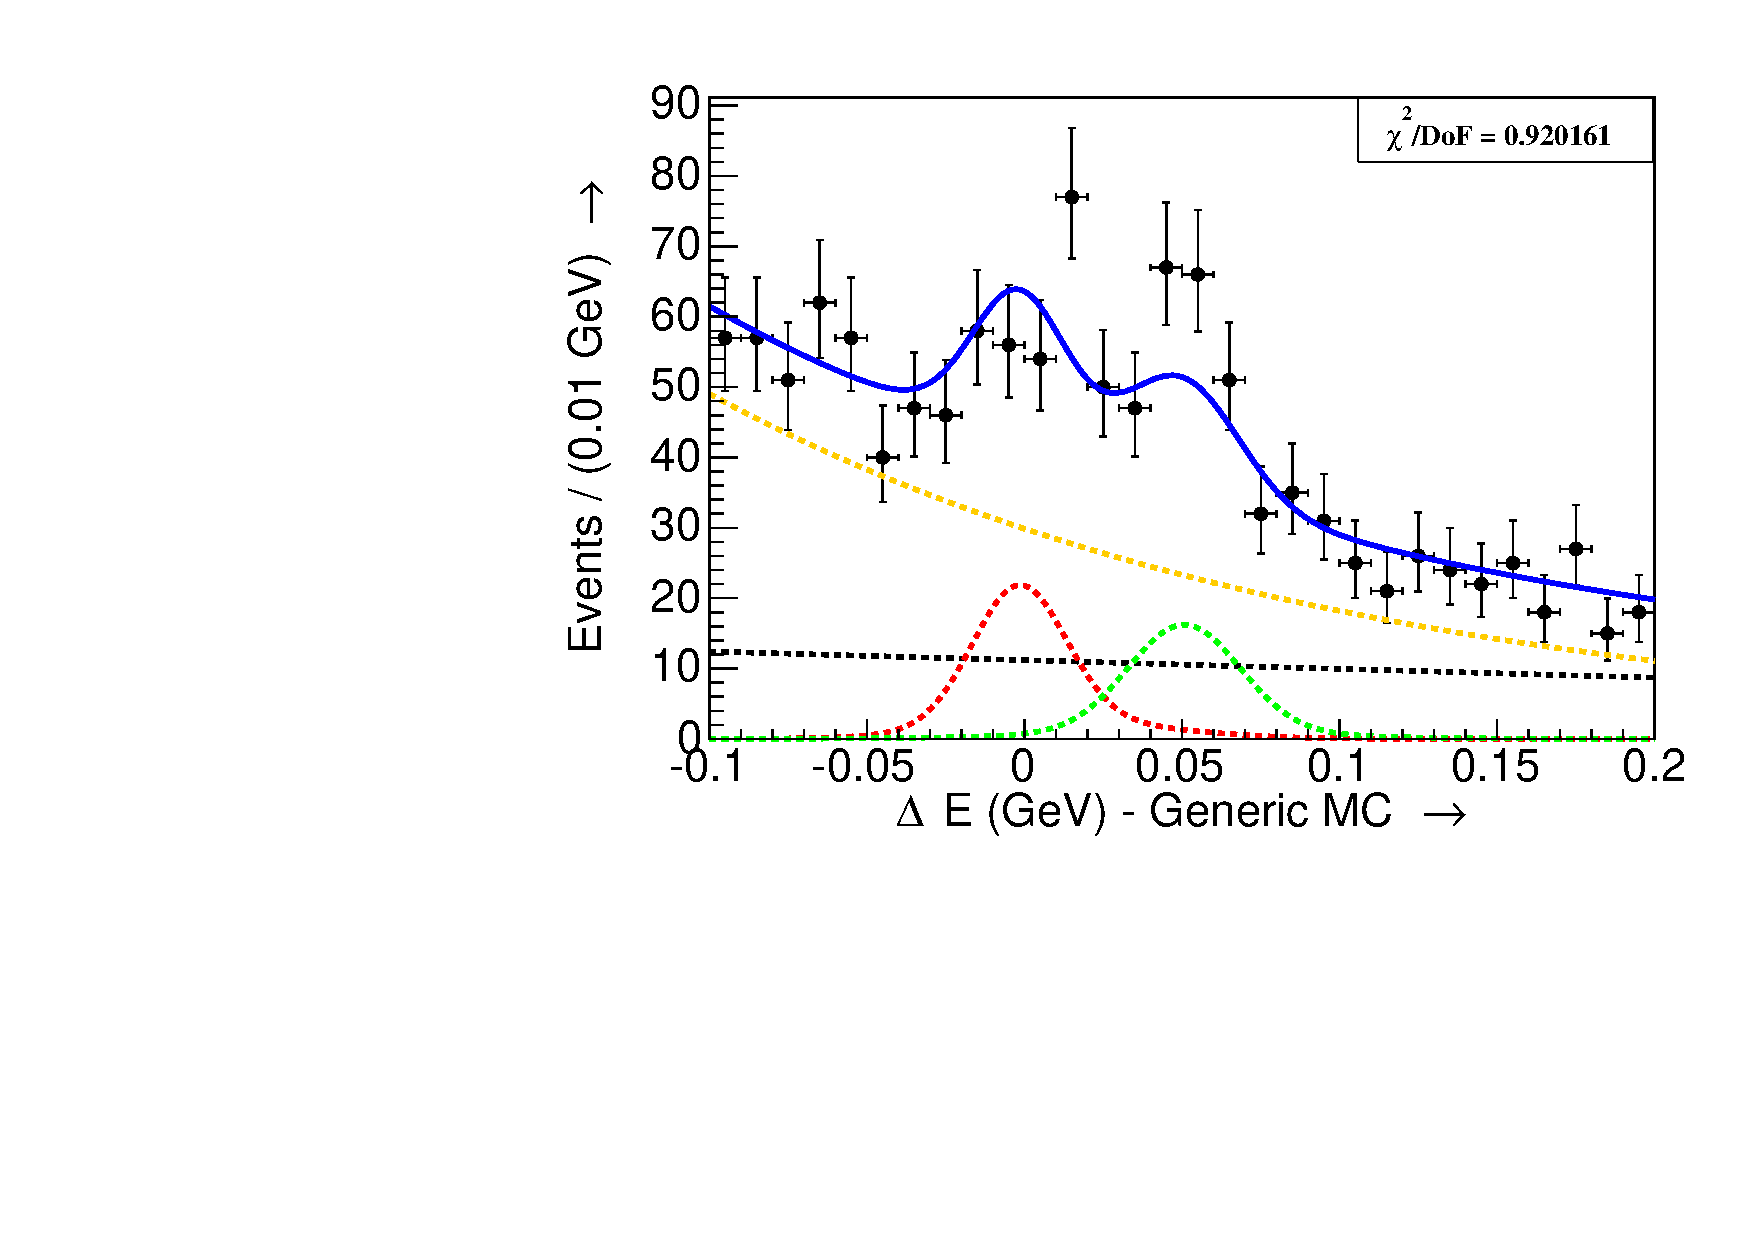
\includegraphics[width=1.5in]{data_DKp_SE.pdf}}\quad
\subfigure[]{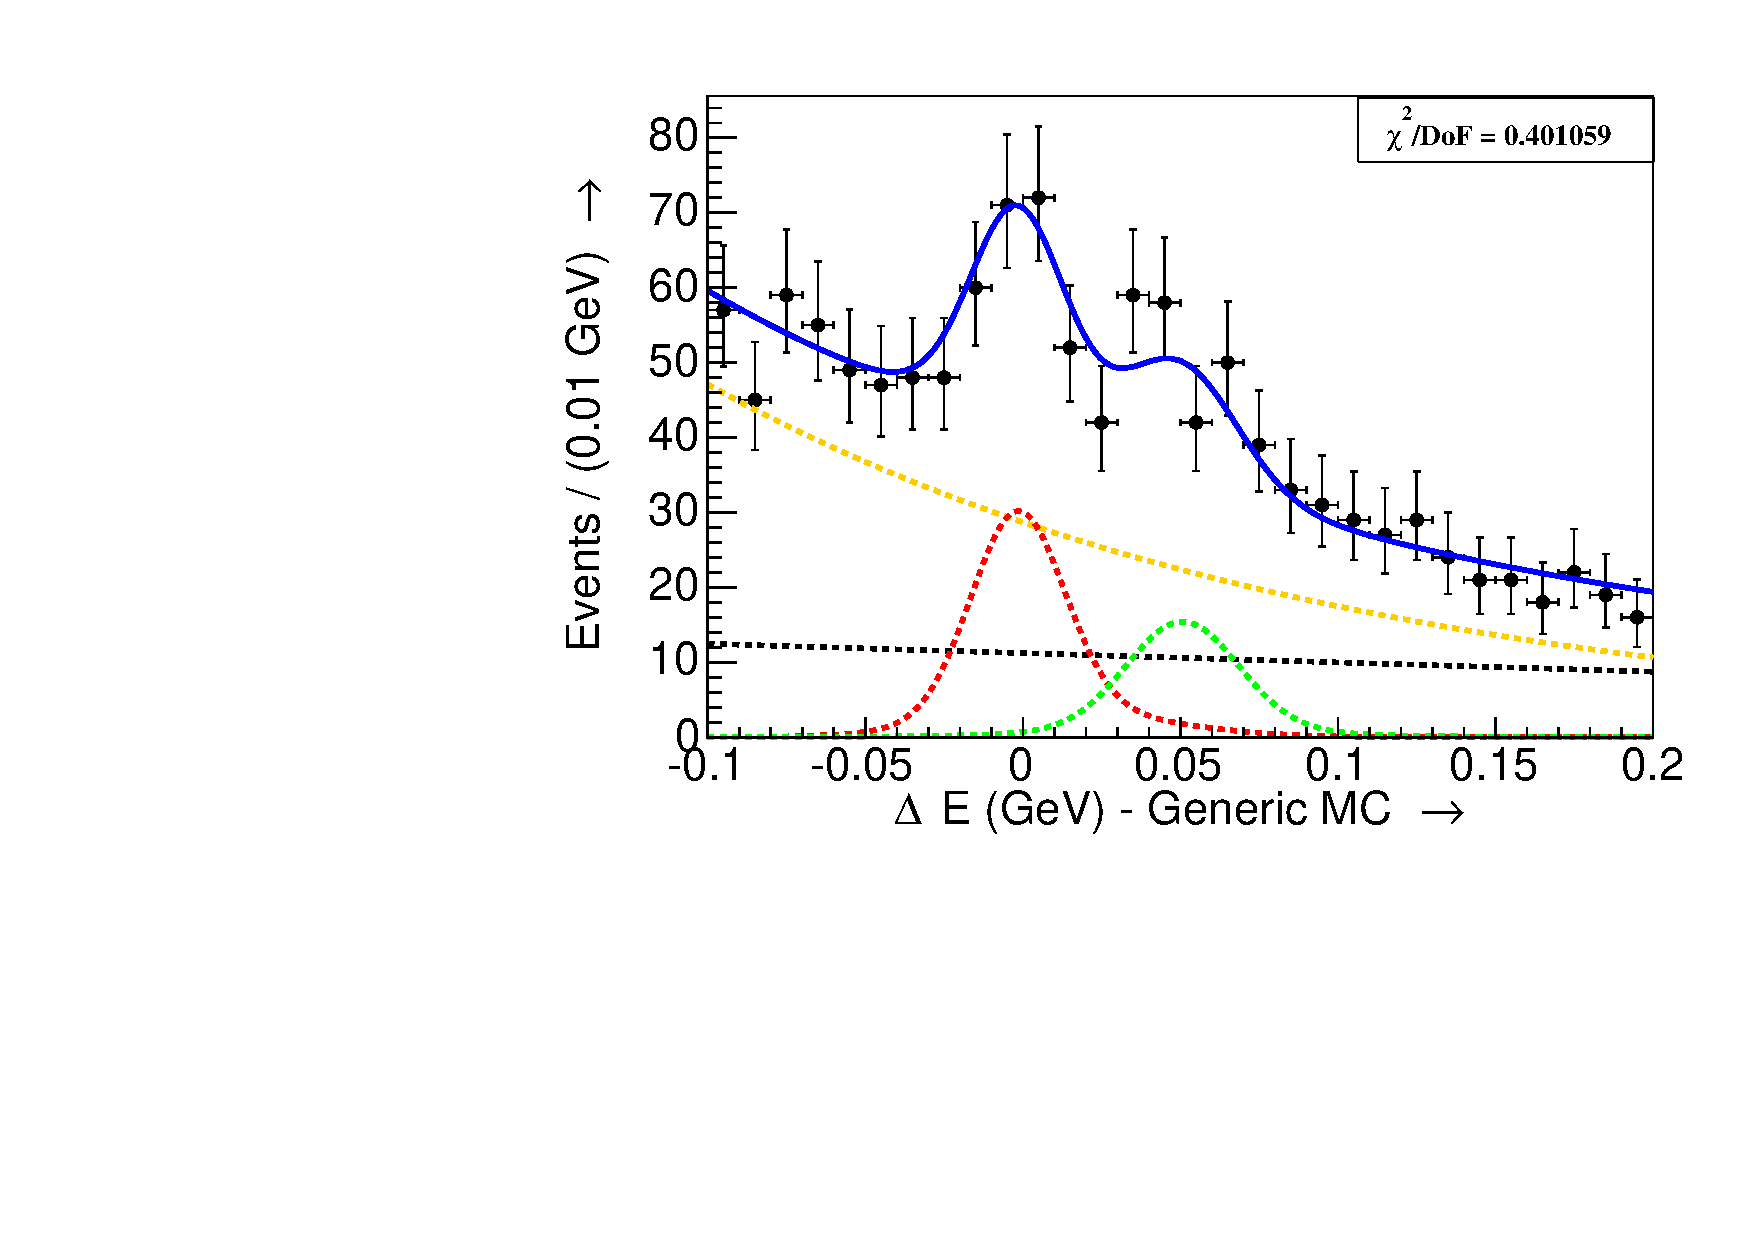
\includegraphics[width=1.5in]{data_DKm_SE.pdf} }}


\caption{Full projections onto $\Delta E$ for $KID < 0.6$ (top row) and $KID > 0.6$ (second row) for the full unblinded Belle dataset. Third row shows signal enhanced ($\mathcal{C}_{NB}' > 2.5$) projections for $KID > 0.6$. The columns denote $\eta = +1$ (left) and $\eta = -1$ (right). The PDFs are signal $D\pi$ (dashed green), signal $DK$ (dashed red), $B\bar{B}$ (dashed orange) and $q\bar{q}$ (dashed black). } \label{fig:Figure 1}
\end{figure} 

The various sources of systematic uncertainties associated with the parameters $A_{F_{+}}$ and $R_{F_{+}}$ are summarised in Table \ref{table:Table 2}, and are estimated as follows. Each of the fixed PDF parameters was varied about its \textit{fixed} value by $\pm 1\sigma$, where $\sigma$ refers to the \textit{statistical} uncertainty in this parameter when it was fixed from a suitable MC sample. In addition to varying the fixed PDF parameters, the $\Delta E$ shape for the $DK$ from $B\bar{B}$ contribution was also varied to a $1^{st}$ order Chebyshev polynomial (as opposed to an exponential). As a result of this change in ansatz shape, there was a $19.66  \%$ ($19.09 \%$) variation in $A_{F_+}$ ($R_{F_{+}}$), which was taken as an additional systematic error.

Possible contribution of unmodelled charmless peaking background ($B^{\pm} \rightarrow K^{\pm}\pi^{\pm}\pi^{\mp}\pi^0$) to the fitted signal yield was estimated by running the fitter on the $M_{D}$ sidebands, $1.1 ~ \mathrm{GeV/}c^2 \leq {\mathrm{M_{D}}} \leq 1.78 ~ \mathrm{GeV/}c^2$ and  $1.923 ~ \mathrm{GeV/}c^2 \leq {\mathrm{M_{D}}} \leq 2.6 ~ \mathrm{GeV/}c^2$. The fitted value of the parameter $N^{D\pi}_{tot}$ is $309 \pm 209$. Applying the formulae from Eq. \ref{eq:5}, and normalizing for the fact that the $M_{D}$ sideband is $9.49$ times wider than the $M_{D}$ signal window, the unmodelled peaking background is $133 \pm 160$ events. We further ran the fitter on the latest rare MC sample, and saw no significant peaking background which could pollute the signal yield. 

We generated an ensemble of 1000 Toy MC experiments from the same 2D PDF used in signal extraction, and ran the fitter on these samples, from which we conclude that any bias in the fitter is small. Further, we performed a linearity test by generating ensembles of Toy MC experiments with the values of $A_{F_+}$ and $R_{F_{+}}$ varied between $-0.2$ to $0.2$ and $0.05$ to $0.10$ respectively (1000 toy experiments at each fixed value of the parameter). Taking the mean fitted value from these ensembles and applying a linear model, we find the slope and intercept for $A_{F_{+}}$ to be $0.989 \pm 0.003$ and $0.0033 \pm 0.0003$ respectively. The corresponding values for $R_{F_{+}}$ are $1.006 \pm 0.002$ and $-0.0014 \pm 0.0002$ respectively. For both parameters, we take the fitted intercept values to be the systematic error contribution from this source. 

In order to study the systematic error contribution from possible crossfeed between $B\bar{B}$ and $q\bar{q}$ yields, we fixed the yields of the $B\bar{B}$ and $q\bar{q}$ components to the truth-matched value in each stream of Generic MC. We then ran the fitter in this configuration and noted the fitted values of $A_{F_{+}}$ and $R_{F_{+}}$. The deviation in $A_{F_{+}}$ and $R_{F_{+}}$ in this constrained fit from their values in the free fit was taken as a systematic error.


\begin{table}[ht]
\caption{Summary of systematic errors in $A_{F_{+}}$ and $R_{F_{+}}$. Here, results are only quoted to 3 decimal places.  }
\centering
\begin{tabular}{c c c} 
\hline\hline
Source of systematic error &  $\Delta A_{F_{+}}^{\mathrm{syst}}$ & $\Delta R_{F_{+}}^{\mathrm{syst}}$  \\
\hline
 & & \\
Fixed PDF parameters & \substack{+0.013 \\ -0.006} & \substack{+0.009 \\ -0.001} \\
 & & \\
Uncertainty in PID efficiency & $\pm 0.000$ &  $\pm 0.000$ \\
 & & \\
Variation of $DK$ from $B\bar{B} \Delta E$ Ansatz shape & $ -0.030$ & $+ 0.014$ \\
 & & \\
Unmodelled peaking background & $\pm 0.044$ & $\pm 0.027$ \\
 & & \\
Fit bias and linearity & $\pm 0.003$  & $\pm 0.001$ \\
 & & \\
Crossfeed between $B\bar{B}$ and $q\bar{q}$ yields & $-0.002$ & $+0.001$ \\
 & & \\
\textbf{Quadrature Sum} & \substack{\boldsymbol{+}\mathbf{0.046} \\ \boldsymbol{-}\mathbf{0.054}} &\substack{\boldsymbol{+}\mathbf{0.032} \\ \boldsymbol{-}\mathbf{0.027}}  \\
\hline
\end{tabular}
\label{table:Table 2}
\end{table}

In summary, an analysis of the decay mode $B^{\pm} \rightarrow [\pi^{+} \pi^{-} \pi^{0}]_{D} K^{\pm}$ using the full Belle dataset was used to determine the CP asymmetry parameter $A_{F_{+}}$ as well as the branching fraction ratio $R_{F_{+}}$. The fitted value of $A_{F_{+}}$ and $R_{F_{+}}$, along with associated statistical and systematic errors are:

\begin{subequations} \label{eq:9}
\begin{align}
&A_{F_{+}} =  0.16 \pm 0.12 (\mathrm{stat.}) \pm 0.05 (\mathrm{syst.}) \nonumber,\\ 
&R_{F_{+}} = 0.076 \pm 0.012 (\mathrm{stat.}) ^{+0.032} _{-0.027} (\mathrm{syst.}) \nonumber ,
\end{align}
\end{subequations}

where the quoted systematic error is the quadrature sum of the various errors evaluated in Table \ref{table:Table 2}. 

The statistical error in the parameter $A_{F_{+}}$ as determined from MC data is comparable to other measurements \cite{BaBar, LHCb}. This analysis will add to the number of modes available for determination of the UT angle $\phi_3$ using the GLW method.


%***** Acknowledgments *****

We thank the KEKB group for the excellent operation of the
accelerator; the KEK cryogenics group for the efficient
operation of the solenoid; and the KEK computer group,
the National Institute of Informatics, and the 
PNNL/EMSL computing group for valuable computing
and SINET5 network support.  We acknowledge support from
the Ministry of Education, Culture, Sports, Science, and
Technology (MEXT) of Japan, the Japan Society for the 
Promotion of Science (JSPS), and the Tau-Lepton Physics 
Research Center of Nagoya University; 
the Australian Research Council;
Austrian Science Fund under Grant No.~P 26794-N20;
the National Natural Science Foundation of China under Contracts 
No.~10575109, No.~10775142, No.~10875115, No.~11175187, No.~11475187, 
No.~11521505 and No.~11575017;
the Chinese Academy of Science Center for Excellence in Particle Physics; 
the Ministry of Education, Youth and Sports of the Czech
Republic under Contract No.~LTT17020;
the Carl Zeiss Foundation, the Deutsche Forschungsgemeinschaft, the
Excellence Cluster Universe, and the VolkswagenStiftung;
the Department of Science and Technology of India; 
the Istituto Nazionale di Fisica Nucleare of Italy; 
the WCU program of the Ministry of Education, National Research Foundation (NRF)
of Korea Grants No.~2011-0029457, No.~2012-0008143,
No.~2014R1A2A2A01005286,
No.~2014R1A2A2A01002734, No.~2015R1A2A2A01003280,
No.~2015H1A2A1033649, No.~2016R1D1A1B01010135, No.~2016K1A3A7A09005603, No.~2016K1A3A7A09005604, No.~2016R1D1A1B02012900,
No.~2016K1A3A7A09005606, No.~NRF-2013K1A3A7A06056592;
the Brain Korea 21-Plus program, Radiation Science Research Institute, Foreign Large-size Research Facility Application Supporting project and the Global Science Experimental Data Hub Center of the Korea Institute of Science and Technology Information;
the Polish Ministry of Science and Higher Education and 
the National Science Center;
the Ministry of Education and Science of the Russian Federation and
the Russian Foundation for Basic Research;
the Slovenian Research Agency;
Ikerbasque, Basque Foundation for Science and
the Euskal Herriko Unibertsitatea (UPV/EHU) under program UFI 11/55 (Spain);
the Swiss National Science Foundation; 
the Ministry of Education and the Ministry of Science and Technology of Taiwan;
and the U.S.\ Department of Energy and the National Science Foundation.
%\begin{verbatim}
 %http://belle.kek.jp/secured/publication/ack.txt
%\end{verbatim}


\begin{thebibliography}{99}


\bibitem{Fplus}
M. Nayak et. al., \emph{First determination of the CP content of $D \rightarrow \pi^+ \pi^- \pi^0$ and $D \rightarrow K^+ K^- \pi^0$}, Phys. Lett. B 740 (2015).

\bibitem{GLW}
M. Gronau, and D. Wyler, \emph{On determining a weak phase from charged B decay asymmetries}, Phys. Lett. B, \textbf{265}(1) 172-176 (1991); M. Gronau and D. London, \emph{How to determine all the angles of the unitary triangle from $B^0_d \rightarrow DK_S$ and $B^0_s \rightarrow D\phi$}, Phys. Lett. B \textbf{253} (1991) 483. 

\bibitem{HFAG} Heavy Flavor Averaging Group, \url{http://www.slac.stanford.edu/xorg/hfag/}.


\bibitem{BaBar}
B. Aubert \textit{et. al.}, \emph{Measurement of the branching fraction and decay rate asymmetry of $B^- \rightarrow D_{\pi^+ \pi^- \pi^0}K^-$}, Phys. Rev. D., \textbf{72}, 071102 (2005)

\bibitem{LHCb}
The LHCb Collaboration, \emph{A study of CP violation in $B^{\mp} \rightarrow Dh^{\mp}$ ($h = K, \pi$) with the modes $D \rightarrow K^{\mp} \pi^{\pm} \pi^0$, $D \rightarrow \pi^{+} \pi^{-} \pi^0$, and $D \rightarrow K^{+} K^{-} \pi^0$}, Phys. Rev. D., \textbf{91}, 112014 (2015)

\bibitem{EvtGen}
The EvtGen Project. \url{http://evtgen.warwick.ac.uk/static/docs/EvtGenGuide.pdf} .

\bibitem{GEANT3}
R. Brun et. al., \emph{GEANT 3 : Users Guide GEANT 3.10, GEANT 3.11 (CERN-DD-EE-84-01), 1984} .

\bibitem{BN1201}
K. Trabelsi and Y. Horii, \emph{Study of $B^- \rightarrow D^{(*)}K^-$ modes for a measurement of $\phi_3$ using ADS and GLW methods}, Belle Note 1201 (v. 3.1) (2011).

\bibitem{BN1271}
M. Nayak, J. Libby, and K. Trabelsi, \emph{Measurements of the branching-fraction ratio and CP-asymmetry in $B^{\pm} \rightarrow [K^{\pm} \pi^{\mp}\pi^0]_DK^{\pm}$ decays}, Belle Note 1271 (v. 2) (2013).

\bibitem{Heller}
A. Heller. \emph{Analysis of the semileptonic decay $B^+ \rightarrow \ell^+ \nu \gamma$ with $\ell^+ = e^+, \mu^+$ at the Belle experiment}. \url{http://ekp-invenio.physik.uni-karlsruhe.de/record/48530/files/EKP-2014-00041.pdf}. Diploma Thesis (2014).

\bibitem{Chris}
J. Libby, G. Wilkinson, and C. Thomas. Private Communication.

\bibitem{Feindt}
M. Feindt, and U. Kerzel, \emph{The NeuroBayes neural network package}. Nucl. Instrum. Methods Phys. Res. Sect. A \textbf{559}(1): 109-194 (2006).

\bibitem{Wolfram}
G.C. Fox and S. Wolfram, \emph{Observables for the Analysis of Event Shapes in $e^+ e^-$ Annihilation and Other Processes}, Phys. Rev. Lett. \textbf{41}, 1581 (1978).

\bibitem{decayTable}
Decay Table b20080331\_1823,  \url{http://belle.kek.jp/group/software/MC/genericmc/b20080331_1823.DECAY.DEC}.

\bibitem{Bdilution}
H. Kakuno \textit{et al.} (Belle Collaboration), Nucl. Instrum. Methods Phys. Res./ Sect. A \textbf{533}, 516 (2004).

\end{thebibliography}
%

\end{document}
